\subsection{Vision Transformer Architecture}

The Vision Transformer (ViT) architecture comprises the following components:

\begin{figure}[htbp]
    \centering
    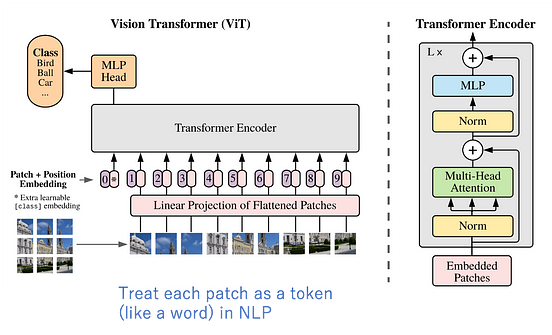
\includegraphics[width=6in]{img/visiontransformer.png}
    \caption{Vision Transformer Architecture}
\end{figure}

\item
\subsubsection{Patch Embedding}
The Patch Embedding step in the Vision Transformer architecture involves the following detailed process:
\\

\noindent a. \textbf{Image Patching:} The input image is divided into a grid of non-overlapping patches.\\
Let $\mathbf{X} \in \mathbf{R}^{H \times W \times C}$ represent the original image, where $H$ is the image height, $W$ is the image width, and $C$ is the number of channels (color depth). We partition $\mathbf{X}$ into patches of size $P \times P \times C$, resulting in a tensor $\mathbf{X}_\text{patches} \in \mathbf{R}^{N \times P \times P \times C}$, where $N$ is the total number of patches.
\\

\noindent b. \textbf{Flattening:} Each patch is reshaped into a vector using a flatten operation. The flattened patches are denoted as $\mathbf{X}_\text{flat} \in \mathbf{R}^{N \times (P \times P \times C)}$.
\\

\noindent c. \textbf{Linear Projection:} The flattened patches are projected into a lower-dimensional space using a learnable linear transformation. Let $\mathbf{W}_\text{proj} \in \mathbf{R}^{(P \times P \times C) \times D_\text{proj}}$ be the projection matrix, where $D_\text{proj}$ is the dimension of the projected space. The projected patch embeddings are computed as $\mathbf{E} = \mathbf{X}_\text{flat} \cdot \mathbf{W}_\text{proj} \in \mathbf{R}^{N \times D_\text{proj}}$.
\\

\noindent d. \textbf{Positional Encoding:} To provide spatial information to the transformer model, positional encodings are added to the patch embeddings. Each patch embedding is enhanced with a positional encoding vector $\mathbf{P} \in \mathbf{R}^{N \times D_\text{proj}}$. The final patch embeddings with positional information are given by $\mathbf{E}_\text{pos} = \mathbf{E} + \mathbf{P}$.

\noindent Mathematically, the above steps can be summarized as follows:

\[
    \mathbf{X}_\text{patches} = \text{ImagePatching}(\mathbf{X}),
\]
\[
    \mathbf{X}_\text{flat} = \text{Flatten}(\mathbf{X}_\text{patches}),
\]
\[
    \mathbf{E} = \mathbf{X}_\text{flat} \cdot \mathbf{W}_\text{proj},
\]
\[
    \mathbf{E}_\text{pos} = \mathbf{E} + \mathbf{P}.
\]

The resulting patch embeddings with positional information, $\mathbf{E}_\text{pos}$, are then used as input for the subsequent stages of the Vision Transformer architecture.


\begin{figure}[htbp]
    \centering
    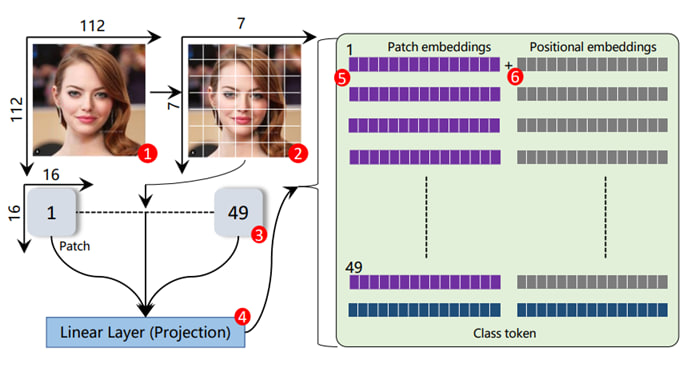
\includegraphics[width=6in]{img/patchembedding.jpg}
    \caption{Patch Embedding}
\end{figure}

\subsubsection{Transformer Encoder}
The patch embeddings are then processed through a stack of transformer encoder layers. Each of these layers consists of two main components: multi-head self-attention and feedforward neural networks.
\\


\noindent \textbf{a. Multi-head self-attention:} This mechanism allows the model to consider relationships between different patches, both locally and globally. It assigns different attention weights to different patches based on their relevance to each other, enabling the model to capture long-range dependencies and relationships within the image. \\
\\
\noindent \textbf{Standard qkv Self-Attention (SA)}:
For an input sequence $z \in \mathbf{R}^{N \times D}$ (with $N$ elements, each having a $D$-dimensional feature vector), we compute a weighted sum over all values $v$ in the sequence. The attention weights $A_{ij}$ are determined based on the similarity between elements of the sequence and their corresponding query $q_i$ and key $k_j$ representations.
\[
    [q, k, v] = zU_{qkv}, \quad U_{qkv} \in \mathbf{R}^{D \times 3Dh}
\]
\[
    A = \text{softmax}\left(\frac{qk^T}{\sqrt{Dh}}\right), \quad A \in \mathbf{R}^{N \times N}
\]
\[
    \text{SA}(z) = Av
\]

MSA extends SA by running $k$ self-attention operations (heads) in parallel and then concatenating their outputs. To ensure consistent computation and parameter complexity, the dimension $Dh$ (from Eq. 5) is usually set to $D/k$.
\[
    \text{MSA}(z) = [SA_1(z); SA_2(z); \ldots ; SA_k(z)], \quad U_{msa} \in \mathbf{R}^{k \cdot Dh \times D}
\]
\begin{figure}[htbp]
    \centering
    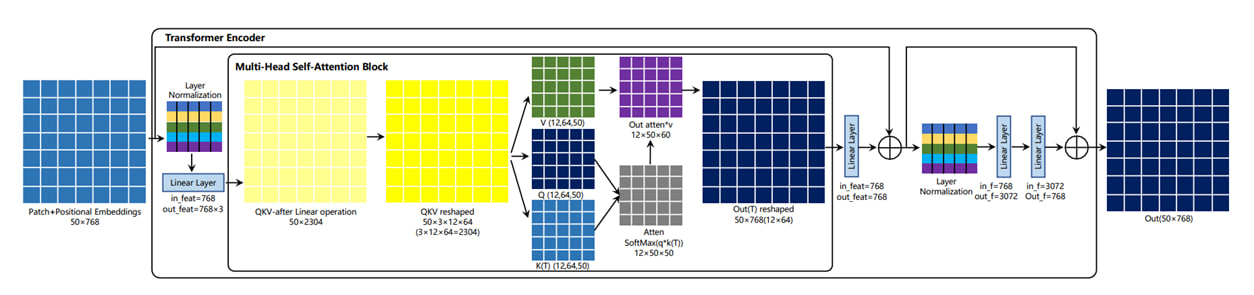
\includegraphics[width=6in]{img/encoderdetails.jpg}
    \caption{Transformer Encoder}
\end{figure}

\noindent \textbf{b. Feedforward neural networks:} After the attention mechanism, the data passes through feedforward neural networks, which process and transform the information further, helping the Vision Transformer model learn intricate features and patterns in the image data.

\noindent Feedforward neural networks consist of multiple layers, including fully connected (dense) layers followed by non-linear activation functions. Let's denote the input to the feedforward neural network as $\mathbf{x} \in \mathbf{R}^{D_{\text{FFN}}}$, where $D_{\text{FFN}}$ is the dimension of the input features.
\\

\noindent The transformation in each layer of the feedforward neural network can be represented as follows:

\[
    \mathbf{h}^{(l+1)} = \text{GELU}\left(\mathbf{W}^{(l)} \mathbf{h}^{(l)} + \mathbf{b}^{(l)}\right),
\]

where $\mathbf{h}^{(l)}$ is the output of the $l$-th layer, $\mathbf{W}^{(l)}$ is the weight matrix, $\mathbf{b}^{(l)}$ is the bias vector, and $\text{GELU}(\cdot)$ is the Gaussian Error Linear Unit activation function.
\\

\noindent The feedforward neural networks in the Vision Transformer's transformer encoder process each patch embedding independently through these layers, capturing complex patterns and relationships within the data.

\noindent After the final feedforward layer, the resulting representations are concatenated and used as the output of the transformer encoder for further processing or downstream tasks, making the Vision Transformer architecture a powerful tool for image analysis and understanding.

\paragraph{Activation Function: Gaussian Error Linear Unit (GELU)}
Activation functions introduce non-linearity, enabling the network to learn and approximate complex, non-linear relationships in the data.
The Gaussian Error Linear Unit (GELU) is an activation function that provides a smooth approximation to the rectifier linear unit (ReLU) activation while maintaining differentiability, which can aid in the training process.

\noindent Two formulations of the GELU function are commonly used:

\[
    \text{GELU}(x) = 0.5x \left(1 + \tanh\left(\frac{\pi}{2} \cdot \left(x + 0.044715x^3\right)\right)\right)
\]

and

\[
    \text{GELU}(x) = \frac{1}{2}x \left(1 + \text{erf}\left(\frac{x}{\sqrt{2}}\right)\right)
\]

Where:
\begin{itemize}
    \item $x$ is the input to the GELU function.
    \item $\text{erf}(z)$ is the error function.
    \item $\pi$ represents the mathematical constant pi.
    \item $\sqrt{2}$ is the square root of 2.
\end{itemize}

The GELU activation function is often used in neural network architectures due to its smoothness and differentiability properties, making it suitable for gradient-based optimization during training.

\noindent Additionally, consider the mathematical expression:
\[
    P(X = c)
\]
where $X$ represents a random variable and $c$ is a constant value. This expression is used to represent the probability that the random variable $X$ takes on the value $c$.
\\
When no activation function is used in a neural network, the model essentially reduces to a linear regression or a linear transformation. Consequently, the entire neural network collapses into a single linear transformation, regardless of the number of layers. This severely limits the expressive power of the network, as it can only learn linear relationships in the data.
\\
\\
Compared to Rectified Linear Unit (ReLU), Exponential Linear Unit (ELU), and Scaled Exponential Linear Unit (SELU), the Gaussian Error Linear Unit (GELU) activation function stands out for its smoothness, handling of negative inputs, and ability to capture complex patterns. 



\subsubsection{Classification Head}
The Classification Head is the final component of the Vision Transformer architecture, responsible for making predictions based on the learned features and patterns from the transformer encoder. It performs classification tasks, such as determining whether an image is real or manipulated.
\\

\noindent \textbf{a. Input Preparation:} After going through the transformer layers, the image is divided into patches and transformed into a useful form for the classification head.
\\

\noindent \textbf{b. Pooling Operation:} Think of this as collecting information from all the patches. The model adds up the important parts from each patch and takes the average. This gives a summary of the whole image.
\\

\noindent \textbf{c. Decision Making:} The model uses this summary to decide what the image might be. For example, it could be deciding if an image is real or fake. It does this by comparing the features it has learned to what it has seen during training.
\\

\noindent \textbf{d. Class Prediction:} The model assigns a score to each possible class (like "real" or "manipulated"). It does this by multiplying the summary with a set of numbers that it learned. Then, it uses the softmax function to turn these scores into probabilities. The class with the highest probability is the final prediction.


\newpage
